% !TeX root = main.tex

\chapter{随机变量及其分布}

\section{随机变量的分布函数}

\subsection{随机变量}

\begin{definition}
    设随机试验 $E$ 的样本空间为 $\varOmega=\{\omega\}$. 如果对于每一个 $\omega\in\varOmega$,都有一个实数 $X(\omega)$ 与之对应,则称 $X=X(\omega)$ 为\textbf{随机变量}(random variable).
\end{definition}

随机变量常用大写字母 $X,Y,Z$ 等表示.

\subsection{分布函数}

\begin{definition}
    设 $X$ 是一个随机变量,对于任意实数 $x$,令 $F(x)=P\{X \leqslant x\}$,称 $F(x)$ 为随机变量 $X$ 的\textbf{分布函数}(cumulative distribution function).
\end{definition}

随机变量 $X$ 的分布函数 $F(x)$ 是定义在 $(-\infty,+\infty)$ 上的函数,是随机事件 $\{X \leqslant x\}$ 发生的概率.分布函数值 $F(a)$ 表示 $X$ 落在区间 $(-\infty,a]$ 上的概率.

\setcounter{propertyname}{0}

\begin{property}
    对于任意实数 $x_1,x_2\, (x_1<x_2)$,有 $P\{x_1 < X \leqslant x_2\}=F(x_2)-F(x_1)$.
\end{property}

\begin{myproof}
    对于任意实数 $x_1,x_2\, (x_1<x_2)$,由于
    $$
    \{x_1 < X \leqslant x_2\} = \{X \leqslant x_2\} - \{X \leqslant x_1\}
    $$
    所以有
    $$
    \begin{aligned}
        P\{x_1 < X \leqslant x_2\} &= P\{X \leqslant x_2\} - P\{X \leqslant x_1\}\\
        &= F(x_2)-F(x_1)
    \end{aligned}
    $$
\end{myproof}

\begin{property}[(单调性)]
    $F(x)$ 是一个单调不减函数.
\end{property}

\begin{myproof}
    对于任意实数 $x_1,x_2\, (x_1<x_2)$,有
    $$
    F(x_2)-F(x_1) = P\{x_1 < X \leqslant x_2\} \geqslant 0
    $$
    因此 $F(x)$ 是单调不减函数.
\end{myproof}

\begin{property}[(有界性)]
    对于任意实数 $x$,有 $0 \leqslant F(x) \leqslant 1$,且
    \begin{gather*}
        F(-\infty)= \lim_{x \to -\infty} F(x)=0\\
        F(+\infty)= \lim_{x \to +\infty} F(x)=1
    \end{gather*}
\end{property}

\begin{myproof}
    因为 $F(x) = P \{ X \leqslant x \}$,根据概率的性质可得 $0 \leqslant F(x) \leqslant 1$.

    $F(x)$ 在 $(-\infty, +\infty)$ 内单调不减且有界,由单调有界原理可知,$\displaystyle\lim_{x \to -\infty} F(x)$ 和 $\displaystyle\lim_{x \to +\infty} F(x)$ 存在.

    记 $A_n = \{ X \leqslant n \}$,则有 $A_n \leqslant A_{n+1}$,$\displaystyle\bigcup_{i=1}^{\infty} A_i = \varOmega$.由海涅定理可得
    $$
    \lim_{x \to +\infty} F(x) = \lim_{n \to \infty} F(n) = \lim_{n \to \infty} P(A_n) = P(\lim_{n \to \infty} A_n) = P(\bigcup_{i=1}^{\infty} A_i) = 1
    $$

    记 $B_n = \{ X \leqslant -n \}$,则有 $B_n \supseteq B_{n+1}$,$\displaystyle\bigcap_{i=1}^{\infty} B_i = \text{\O}$.由海涅定理可得
    $$
    \lim_{x \to -\infty} F(x) = \lim_{n \to \infty} F(-n) = \lim_{n \to \infty} P(B_n) = P(\lim_{n \to \infty} B_n) = P(\bigcap_{i=1}^{\infty} B_i) = 0
    $$
\end{myproof}

\begin{property}[(右连续性)]
    $F(x)$ 处处右连续,即 $F(x^+)=F(x)$.
\end{property}

\begin{myproof}
    因为 $F(x)$ 是单调不减有界函数,所以对任意实数 $x_0$,右极限 $F(x_0^+)$ 一定存在.记 $A_n = \{ X \leqslant x_0 + \dfrac{1}{n} \}$,则有 $A_n \supseteq A_{n+1}$,$\displaystyle\bigcap_{i=1}^{\infty} A_i = \{ X \leqslant x_0 \}$,由海涅定理得
    $$
    \begin{aligned}
        \lim_{x \to x_0^+} F(x) &= \lim_{n \to \infty} F(x_0 + \dfrac{1}{n}) \\
        &= \lim_{n \to \infty} P(A_n) \\
        &= P(\lim_{n \to \infty} A_n) \\
        &= P(\bigcap_{i=1}^{\infty} A_i) \\
        &= P \{ X \leqslant x_0 \} \\
        &= F(x_0)
    \end{aligned}
    $$
\end{myproof}

单调性、有界性、右连续性是分布函数的基本性质.分布函数一定具有这些基本性质,反过来,满足这些基本性质的函数一定是某个随机变量的分布函数.因此,这三条基本性质是判定某个函数能否成为分布函数的充分必要条件.

\section{离散型随机变量及其概率分布}

\begin{definition}
    如果一个随机变量 $X$ 所有可能取到的不相同的值是有限个或可列无限多个,并且以确定的概率取这些不同的值,则称 $X$ 为\textbf{离散型随机变量}(discrete random variable).
\end{definition}

\begin{definition}
    设离散型随机变量 $X$ 所有可能取的值为 $x_k\, (k=1,2,\cdots)$,$X$ 取各个可能值的概率,即事件 $\{X=x_k\}$ 的概率为
    \begin{equation} \label{equation:distribution}
        P\{X=x_k\} = p_k \quad k=1,2,\cdots
    \end{equation}
    并且 $p_k$ 满足以下两个条件:
    \begin{enumerate}
        \item 非负性:$p_k \geqslant 0$;\vspace{0.5em}
        \item 归一性:$\displaystyle\sum_{k=1}^\infty p_k=1$,
    \end{enumerate} \vspace{0.5em}
    则称式 \eqref{equation:distribution} 为离散型随机变量 $X$ 的\textbf{概率分布}(probability distribution)或\textbf{分布律}.
\end{definition}

概率分布也可以用如下的表格来表示:
\begin{table*}[htbp]
    \centering

    \begin{tabular}{c | c c c c c}
        \hline
        $X$ & $x_1$ & $x_2$ & $\cdots$ & $x_k$ & $\cdots$ \\
        \hline
        $P$ & $p_1$ & $p_2$ & $\cdots$ & $p_k$ & $\cdots$ \\
        \hline
    \end{tabular}
\end{table*}

概率分布反映了离散型随机变量的统计规律性.

对于任意实数 $x$,随机事件 $\{X \leqslant x\}$ 可以表示成 $\displaystyle\bigcup_{x_k \leqslant x} \{X=x_k\}$. 由于 $x_k\, (k=1,2,\cdots)$ 互不相同,根据概率的可加性,可得离散型随机变量 $X$ 的分布函数为
$$
F(x) = P\{X \leqslant x\} = \sum_{x_k \leqslant x} P\{X=x_k\} = \sum_{x_k \leqslant x} p_k
$$

\section{连续型随机变量及其概率密度}

\begin{definition} \label{def:f(x)}
    对于随机变量 $X$ 的分布函数 $F(x)$,如果存在非负函数 $f(x)$,使得对任意的 $x$,都有 $F(x)=\displaystyle\int_{-\infty}^x f(t)\,\text{d}t$,则称随机变量 $X$ 是\textbf{连续型随机变量}(continuous random variable),其中函数 $f(x)$ 叫做 $X$ 的\textbf{概率密度函数}(probability density function),简称为\textbf{概率密度}(probability density),记作 $X \sim f(x)$.
\end{definition}

由定义 \ref{def:f(x)} 可知,连续型随机变量的分布函数处处连续.

概率密度 $f(x)$ 的性质如下.

\setcounter{propertyname}{0}

\begin{property} \label{prop:f(x)>=0}
    $f(x) \geqslant 0$
\end{property}

\begin{property} \label{prop:f(x):integral=1}
    $\displaystyle\int_{-\infty}^{+\infty} f(x)\,\text{d}x = 1$
\end{property}

满足性质 \ref*{prop:f(x)>=0} 与性质 \ref*{prop:f(x):integral=1} 的函数 $f(x)$ 必然是某随机变量的概率密度.

\begin{property}
    对于任意实数 $a,b\,(a<b)$,有
    $$
    P\{a < X \leqslant b\}=F(b)-F(a)=\int_a^b f(x)\,\text{d}x
    $$
\end{property}

由以上性质可知,概率密度曲线总是位于 $x$ 轴上方,并且介于它和 $x$ 轴之间的面积等于 1;随机变量落在区间 $(a,b]$ 的概率 $P\{a < X \leqslant b\}$ 等于区间 $(a,b]$ 上曲线 $y=f(x)$ 之下的曲边梯形的面积.

\begin{property} \label{prop:F'(x)=f(x)}
    如果 $f(x)$ 在点 $x$ 处连续,则有 $F'(x)=f(x)$.
\end{property}

由性质 \ref*{prop:F'(x)=f(x)} 可知,在 $f(x)$ 的连续点有
$$
\begin{aligned}
    f(x) &= \lim_{\Delta x \to 0^+} \dfrac{F(x + \Delta x)-F(x)}{\Delta x}\\
    &= \lim_{\Delta x \to 0^+} \dfrac{P\{x < X \leqslant x + \Delta x\}}{\Delta x}
\end{aligned}
$$
可见概率密度反映了随机变量在点 $x$ 处概率分布的密集程度.$f(x)$ 的大小能反映出随机变量 $X$ 在点 $x$ 附近取值的可能性大小,即概率的大小.因此,用概率密度描述连续型随机变量的分布比用分布函数更直观.当不考虑高阶无穷小时,有
$$
P\{x < X \leqslant x + \Delta x\} \approx f(x) \Delta x
$$

\begin{conclusion}
    连续型随机变量取任意指定实数的概率均为零.
\end{conclusion}

\begin{myproof}
    对于 $X$ 的任意一个可取的值 $x$,设 $\Delta x > 0$,由于事件 $\{X=x\} \subseteq \{x - \Delta x < X \leqslant x\}$,因此有
    $$
    0 \leqslant P\{X=x\} \leqslant P\{x - \Delta x < X \leqslant x\} = F(x)-F(x-\Delta x)
    $$
    令 $\Delta x \to 0$,可得
    $$
    P\{X=x\}=0
    $$
    因此,连续型随机变量取任意指定实数的概率均为零.
\end{myproof}


据此,在计算连续型随机变量在某一区间取值的概率时,可以不区分该区间是开区间或闭区间或半开半闭区间,即有
$$
P\{x_1 < X < x_2\} = P\{x_1 \leqslant X \leqslant x_2\} = P\{x_1 < X \leqslant x_2\} = P\{x_1 \leqslant X < x_2\} = \int_{x_1}^{x_2} f(x)\,\text{d}x
$$

由上述结论可知,概率为 0 的事件未必是不可能事件,概率为 1 的事件也未必是必然事件.

\section{常用的分布}

\subsection{(0-1)分布}

\begin{definition}
    如果离散型随机变量 $X$ 只取 0 与 1 两个值,其概率分布为
    $$
    P\{X=0\}=1-p, \; P\{X=1\}=p, \; 0<p<1
    $$
    或写成
    $$
    P\{X=k\}=p^k (1-p)^{1-k}, \; k=0,1, \; 0<p<1
    $$
    则称随机变量 $X$ 服从参数为 $p$ 的\textbf{(0-1)分布}或\textbf{两点分布}(two-point distribution).
\end{definition}

服从两点分布的随机变量 $X$ 的概率分布也可以写成
\begin{table*}[htbp]
    \centering

    \begin{tabular}{c | c c}
        \hline
        $X$ & 0 & 1 \\
        \hline
        $P$ & $1-p$ & $p$ \\
        \hline
    \end{tabular}
\end{table*}

\subsection{二项分布}

在 $n$ 重伯努利试验中,如果以 $X$ 表示事件 $A$ 出现的次数,则 $X$ 是一个离散型随机变量,它的所有可能取值是 $0,1,2,\cdots,n$.设 $P(A)=p\,(0<p<1)$,则由二项概率公式(式 \eqref{equation:binomial})可得
$$
P\{X=k\}=C_n^k p^k (1-p)^{n-k}, \; k=0,1,\cdots,n
$$

\begin{definition} \label{def:binomial distribution}
    如果随机变量 $X$ 的概率分布为
    $$
    P\{X=k\}=C_n^k p^k (1-p)^{n-k}, \; k=0,1,\cdots,n
    $$
    则称随机变量 $X$ 服从参数为 $n,p$ 的\textbf{二项分布}(binomial distribution),记作 $X \sim B(n,p)$.
\end{definition}

由定义 \ref{def:binomial distribution} 可得
\begin{gather*}
    P\{X=k\} \geqslant 0\\
    \sum_{k=0}^n P\{X=k\} = \sum_{k=0}^n C_n^k p^k (1-p)^{n-k} = [p+(1-p)]^n=1
\end{gather*}

特别地,当 $n=1$ 时,二项分布 $B(1,p)$ 的概率分布为
$$
P\{X=k\} = p^k (1-p)^{1-k}, \; k=0,1
$$
这就是(0-1)分布. 因此,(0-1)分布是二项分布的特例.

\subsection{泊松分布}

\begin{definition}
    如果离散型随机变量 $X$ 的所有可能取值为 $0,1,2,\cdots$,并且
    $$
    P\{X=k\} = \dfrac{\lambda^k e^{-\lambda}}{k!}, \; k=0,1,2\cdots
    $$
    其中 $\lambda > 0$ 是常数,则称随机变量 $X$ 服从参数为 $\lambda$ 的\textbf{泊松分布}(poisson distribution),记作 $X \sim P(\lambda)$ 或 $X \sim \pi(\lambda)$.
\end{definition}

易知
\begin{gather*}
    \dfrac{\lambda^k e^{-\lambda}}{k!} > 0\\
    \sum_{k=0}^\infty \dfrac{\lambda^k e^{-\lambda}}{k!} = e^{-\lambda} \sum_{k=0}^\infty \dfrac{\lambda^k}{k!} = e^{-\lambda} e^{\lambda}=1
\end{gather*}

\begin{figure}[htbp]
    \centering

    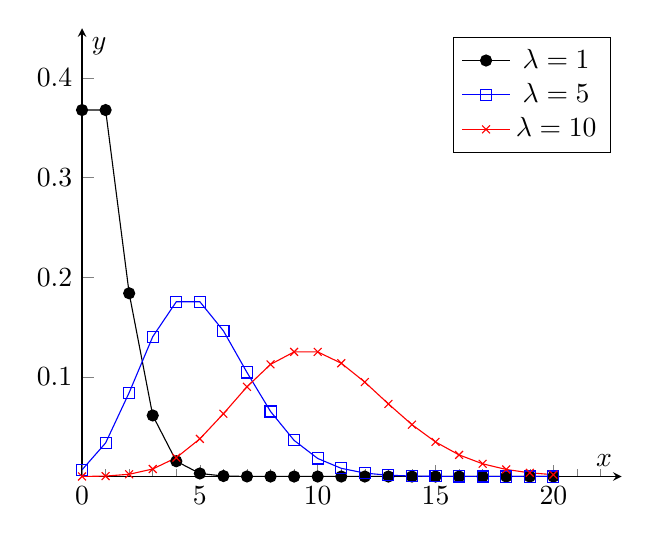
\begin{tikzpicture}
        \begin{axis}[xlabel=$x$, ylabel=$y$,
            axis lines=center,
            tick align=inside,
            xtick distance=5, ytick distance=0.1,
            minor x tick num=4,
            extra x ticks={0},
            xmin=0, xmax=22.9,
            ymin=0, ymax=0.45]
            \addplot[domain=0:20, samples=21, mark=*]{exp(-1)/(x!)};
            \addplot[domain=0:20, samples=21, mark=square, color=blue]{5^x * exp(-5) / (x!)};
            \addplot[domain=0:20, samples=21, mark=x, color=red]{10^x * exp(-10) / (x!)};

            \legend{$\lambda=1$, $\lambda=5$, $\lambda=10$}
        \end{axis}
    \end{tikzpicture}

    \caption{泊松分布}
\end{figure}

\begin{theorem}[(泊松定理)]
    设 $\lambda > 0$ 是常数,$n$ 为任意正整数,$n p_n=\lambda$,则对任一固定的非负整数 $k$,有
    $$
    \lim_{n\to\infty} C_n^k p_n^k (1-p_n)^{n-k} = \dfrac{\lambda^k e^{-\lambda}}{k!}
    $$
\end{theorem}

\begin{myproof}
    因为 $n p_n=\lambda$,故 $p_n=\dfrac{\lambda}{n}$,从而对于任意固定的非负整数 $k$,有
    $$
    \begin{aligned}
        & C_n^k p_n^k (1-p_n)^{n-k}\\
        =\ & \dfrac{n(n-1) \cdots (n-k+1)}{k!} \left( \dfrac{\lambda}{n} \right)^k \left( 1-\dfrac{\lambda}{n} \right)^{n-k}\\
        =\ & \dfrac{\lambda^k}{k!} \left[ 1 \times \left( 1-\dfrac{1}{n} \right) \left( 1-\dfrac{2}{n} \right) \cdots \left( 1-\dfrac{k-1}{n} \right) \right] \left( 1-\dfrac{\lambda}{n} \right)^n \left( 1-\dfrac{\lambda}{n} \right)^{-k}
    \end{aligned}
    $$
    对于固定的 $k$,有
    $$
    \begin{aligned}
        & \lim_{n \to \infty} 1 \times \left( 1-\dfrac{1}{n} \right) \left( 1-\dfrac{2}{n} \right) \cdots \left( 1-\dfrac{k-1}{n} \right) \to 1 \\
        & \lim_{n \to \infty} \left( 1-\dfrac{\lambda}{n} \right)^n \to e^{-\lambda} \\
        & \lim_{n \to \infty} \left( 1-\dfrac{\lambda}{n} \right)^{-k}\to 1
    \end{aligned}
    $$
    所以
    $$
    \lim_{n\to\infty} C_n^k p_n^k (1-p_n)^{n-k} = \dfrac{\lambda^k e^{-\lambda}}{k!}
    $$
\end{myproof}

由于 $n p_n=\lambda$,意味着当 $n$ 很大时 $p_n$ 必定很小.因此,泊松定理表明,当 $n$ 很大而 $p$ 很小时,有下面的近似公式
$$
C_n^k p^k (1-p)^{n-k}\approx \dfrac{\lambda^k e^{-\lambda}}{k!}
$$
其中 $\lambda=np$.也就是说,对于二项分布 $B(n,p)$,当 $n$ 很大而 $p$ 很小时,近似为泊松分布 $P(np)$.

\subsection{几何分布}

设试验 $E$ 只有两个对立的结果 $A$ 和 $\overline{A}$,并且 $P(A)=p, \, P(\overline{A})=1-p$,其中 $0<p<1$. 将试验 $E$ 独立地重复进行下去,直到事件 $A$ 发生为止. 如果用 $X$ 表示所需要的试验次数,则 $X$ 是一个随机变量,它可能取的值是 $1,2,3,\cdots$. $X$ 的概率分布为
$$
P\{X=k\}=(1-p)^{k-1} p, \; k=1,2,\cdots
$$
称随机变量 $X$ 服从参数为 $p$ 的\textbf{几何分布}(geometric distribution).

易知
\begin{gather*}
    (1-p)^{k-1} p > 0\\
    \sum_{k=1}^\infty (1-p)^{k-1} p = p \sum_{i=0}^\infty (1-p)^i = p \cdot \dfrac{1}{1-(1-p)} = 1    
\end{gather*}
\newline

\subsection{均匀分布}

\begin{definition}
    如果连续型随机变量 $X$ 的概率密度为
    $$
    f(x)=\begin{cases}
        \dfrac{1}{b-a} & a<x<b \\[0.5em]
        0 & \text{其他}
    \end{cases}
    $$
    则称 $X$ 在区间 $(a,b)$ 上服从\textbf{均匀分布}(uniform distribution),记作 $X \sim U(a,b)$.
\end{definition}

若 $X \sim U(a,b)$,则 $X$ 的分布函数为
$$
F(x)=\begin{cases}
    0 & x<a \\[0.2em]
    \dfrac{x-a}{b-a} & a \leqslant x < b \\[0.5em]
    1 & x \geqslant b
\end{cases}
$$

\begin{figure}[htbp]
    \centering

    \subfigure[均匀分布的概率密度]{
        \centering
        \begin{tikzpicture}[>=Stealth]
            % 坐标轴
            \draw[->] (-1, 0)--(3, 0) node[below]{$x$};
            \draw[->] (0, -1)--(0, 2.5) node[left]{$f(x)$};
            \node at (0, 0) [below right] {$O$};
            % 定义端点
            \coordinate (m) at (-0.5, 1);
            \coordinate (n) at (2.5, 1);
            % 曲线
            \draw[line width=1.5pt] (m)--(n);
            \draw[line width=1.5pt] (-1, 0)--(-0.5, 0);
            \draw[line width=1.5pt] (2.5, 0)--(2.85,0);
            % 标记点
            \fill (-0.5, 0) node[below]{$a$} circle (2pt);
            \fill (2.5, 0) node[below]{$b$} circle (2pt);
            \node at (m) [dot] {};
            \node at (n) [dot] {};
            \node at (0, 1) [above right] {$\dfrac{1}{b-a}$};
        \end{tikzpicture}
    }
    \subfigure[均匀分布的分布函数]{
        \centering
        \begin{tikzpicture}[>=Stealth]
            % 坐标轴
            \draw[->] (-1, 0)--(4, 0) node[below]{$x$};
            \draw[->] (0, -1)--(0, 2.5) node[left]{$F(x)$};
            \node at (0, 0) [below right] {$O$};
            % 曲线
            \draw[line width=1.5pt] (-1, 0) -- (-0.5, 0) node[below]{$a$} -- (2.5, 1) -- (3.5, 1);
            % 标记点
            \node at (0, 1) [left] {$1$};
            \node at (2.5, 0) [below] {$b$};
            % 辅助线
            \draw[dashed] (0, 1)--(2.5, 1)--(2.5, 0);
        \end{tikzpicture}
    }

    \caption{}
\end{figure}

对任意的两个数 $x_1, x_2 \in (a,b)$,如果 $x_1 < x_2$,则有
$$
P\{x_1 \leqslant X \leqslant x_2\} = \int_{x_1}^{x_2} \dfrac{\text{d}x}{b-a} = \dfrac{x_2-x_1}{b-a}
$$
这说明随机变量 $X$ 位于区间 $(a,b)$ 的任一子区间 $[x_1,x_2]$ 内的概率,只依赖于子区间 $[x_1,x_2]$ 的长度,而与子区间的位置无关.

\subsection{指数分布}

\begin{definition}
    如果连续型随机变量 $X$ 的概率密度为
    $$
    f(x)=\begin{cases}
        \lambda e^{-\lambda x} & x>0 \\
        0 & x \leqslant 0
    \end{cases}
    $$
    其中 $\lambda>0$ 是常数,则称 $X$ 服从参数为 $\lambda$ 的\textbf{指数分布}(exponential distribution).
\end{definition}

服从指数分布的随机变量 $X$ 的分布函数为
$$
F(x)=\begin{cases}
    0 & x \leqslant 0 \\
    1-e^{-\lambda x} & x>0
\end{cases}
$$

\begin{figure}[htbp]
    \centering

    \subfigure[指数分布的概率密度]{
        \centering
        \begin{tikzpicture}[>=Stealth]
            % 坐标轴
            \draw[->] (-1, 0)--(3.5, 0) node[below]{$x$};
            \draw[->] (0, -1)--(0, 2) node[left]{$f(x)$};
            \node at (0, 0) [below left] {$O$};
            % 曲线
            \draw[domain=0:3, line width=1.5pt] plot (\x, {exp(-1 * \x)});
            \draw[line width=1.5pt] (-1, 0)--(0, 0);
            % 标记点
            \node at (0, 1) [dot, label={left: $\lambda$}] {};
            \fill (0, 0) circle (2pt);
        \end{tikzpicture}
    }
    \subfigure[指数分布的分布函数]{
        \centering
        \begin{tikzpicture}[>=Stealth]
            % 坐标轴
            \draw[->] (-1, 0)--(3.5, 0) node[below]{$x$};
            \draw[->] (0, -1)--(0, 2) node[left]{$F(x)$};
            \node at (0, 0) [below left] {$O$};
            % 曲线
            \draw[domain=0:3, line width=1.5pt] plot (\x, {1 - exp(-1 * \x)});
            \draw[line width=1.5pt] (-1, 0)--(0, 0);
            % 辅助线
            \draw[dashed] (0, 1) node[left]{$1$} -- (3.2, 1);
        \end{tikzpicture}
    }

    \caption{}
\end{figure}

\subsection{正态分布}

\subsubsection{正态分布及其性质}

\begin{definition}
    如果连续型随机变量 $X$ 的概率密度为
    $$
    f(x) = \dfrac{1}{\sqrt{2\pi} \sigma} e^{-\frac{(x-\mu)^2}{2\sigma^2}}, \; -\infty < x < +\infty
    $$
    其中 $\mu,\sigma \, (\sigma>0)$ 为常数,则称 $X$ 服从参数为 $\mu,\sigma$ 的\textbf{正态分布},记作 $X \sim N(\mu,\sigma^2)$.
\end{definition}

若 $X \sim N(\mu,\sigma^2)$,则 $X$ 的分布函数为
$$
F(x) = \dfrac{1}{\sqrt{2\pi} \sigma} \int_{-\infty}^x e^{-\frac{(t-\mu)^2}{2\sigma^2}} \, \text{d}t, \; -\infty < x < +\infty
$$

\begin{figure}[htbp]
    \centering

    \subfigure[正态分布的概率密度]{
        \centering
        \begin{tikzpicture}[>=Stealth, yscale=5]
            % 定义变量
            \def\Mu{2}
            \def\Sigma{1}
            % 坐标轴
            \draw[->] (\Mu-3*\Sigma-0.5, 0)--(\Mu+3*\Sigma+0.5, 0) node[below]{$x$};
            \draw[->] (0, -0.2)--(0, 0.6) node[right]{$f(x)$};
            \node at (0, 0) [below left] {$O$};
            % 曲线
            \draw[domain=\Mu-3*\Sigma:\Mu+3*\Sigma, line width=1.5pt, smooth] plot (\x, {exp(-1 * pow(\x-\Mu, 2) / (2*\Sigma*\Sigma)) / (sqrt(2*pi)*\Sigma)});
            % 辅助线
            \draw[dashed] (0, {1/(sqrt(2*pi)*\Sigma)}) node[left]{$\dfrac{1}{\sqrt{2 \pi} \sigma}$} -- (\Mu, {1/(sqrt(2*pi)*\Sigma)}) -- (\Mu, 0) node[below]{$\mu$};
            \draw[dashed] (\Mu-\Sigma, 0) node[below]{$\mu-\sigma$} -- (\Mu-\Sigma, {exp(-0.5) / (sqrt(2*pi)*\Sigma)});
            \draw[dashed] (\Mu+\Sigma, 0) node[below]{$\mu+\sigma$} -- (\Mu+\Sigma, {exp(-0.5) / (sqrt(2*pi)*\Sigma)});
        \end{tikzpicture}
    }
    \subfigure[正态分布的分布函数]{
        \centering
        \begin{tikzpicture}[>=Stealth, yscale=2]
            % 定义变量
            \def\Mu{2}
            \def\Sigma{1}
            % 坐标轴
            \draw[->] (-1, 0)--(5, 0) node[below]{$x$};
            \draw[->] (0, -0.5)--(0, 1.5) node[left]{$F(x)$};
            \node at (0, 0) [below left] {$O$};
            % 曲线
            \draw[domain=-0.5:4.5, line width=1.5pt, smooth] plot (\x, {1 / (1+exp(-1.70174454109 * (\x-\Mu)))});
            % 辅助线
            \draw[dashed] (0, 1) node[left]{$1$} -- (4.7, 1);
            \draw[dashed] (0, 0.5) node[left]{$0.5$} -- (\Mu, 0.5) -- (\Mu, 0) node[below]{$\mu$};
        \end{tikzpicture}
    }

    \vspace{-1em}

    \caption{}
\end{figure}

概率密度曲线 $y=f(x)$ 关于直线 $x=\mu$ 对称,并在 $x=\mu$ 处取得最大值 $\dfrac{1}{\sqrt{2\pi}\sigma}$,在横坐标 $x=\mu\pm\sigma$ 处有拐点,以 $x$ 轴为水平渐近线.

如果固定 $\sigma$,改变 $\mu$ 的值,则概率密度曲线沿着 $x$ 轴平移,但形状不变,如图 \ref{fig:mu} 所示.

\begin{figure}[htbp]
    \centering

    \begin{tikzpicture}[>=Stealth, yscale=3.5]
        % 定义变量
        \def\Mu{2}
        \def\Sigma{0.7}
        \def\xMu{4.5}
        % 坐标轴
        \draw[->] (\Mu-3*\Sigma-0.5, 0)--(\xMu+3*\Sigma+0.5, 0) node[below]{$x$};
        \draw[->] (0, -0.2)--(0, 0.8) node[right]{$f(x)$};
        \node at (0, 0) [below left] {$O$};
        % 曲线
        \draw[domain=\Mu-3*\Sigma:\Mu+3*\Sigma, line width=1.5pt, smooth] plot (\x, {exp(-1 * pow(\x-\Mu, 2) / (2*\Sigma*\Sigma)) / (sqrt(2*pi)*\Sigma)});
        \draw[domain=\xMu-3*\Sigma:\xMu+3*\Sigma, line width=1.5pt, smooth] plot (\x, {exp(-1 * pow(\x-\xMu, 2) / (2*\Sigma*\Sigma)) / (sqrt(2*pi)*\Sigma)});
        % 辅助线
        \draw[dashed] (\Mu, {1/(sqrt(2*pi)*\Sigma)}) -- (\Mu, 0) node[below]{$\mu_1$};
        \draw[dashed] (\xMu, {1/(sqrt(2*pi)*\Sigma)}) -- (\xMu, 0) node[below]{$\mu_2$};
    \end{tikzpicture}

    \vspace{-1em}

    \caption{}
    \label{fig:mu}
\end{figure}

如果固定 $\mu$,改变 $\sigma$ 的值,则由 $y_{\text{max}}=\dfrac{1}{\sqrt{2\pi}\sigma}$ 可知:$\sigma$ 越小,概率密度曲线在 $x=\mu$ 附近越陡峭,$X$ 落在 $x=\mu$ 附近的概率越大;$\sigma$ 越大,概率密度曲线越平坦.如图 \ref{fig:sigma} 所示.

\begin{figure}[htbp]
    \centering

    \begin{tikzpicture}[>=Stealth, yscale=4]
        % 定义变量
        \def\Mu{2}
        \def\Sigma{1}
        \def\sSigma{0.5}
        \def\tSigma{2}
        % 坐标轴
        \draw[->] (\Mu-2*\tSigma-0.5, 0)--(\Mu+2*\tSigma+0.5, 0) node[below]{$x$};
        \draw[->] (0, -0.2)--(0, 0.9) node[right]{$f(x)$};
        \node at (0, 0) [below left] {$O$};
        % 曲线
        \draw[domain=\Mu-3*\Sigma:\Mu+3*\Sigma, line width=1.5pt, smooth] plot (\x, {exp(-1 * pow(\x-\Mu, 2) / (2*\Sigma*\Sigma)) / (sqrt(2*pi)*\Sigma)});
        \draw[domain=\Mu-3*\sSigma:\Mu+3*\sSigma, line width=1.5pt, draw=red, smooth] plot (\x, {exp(-1 * pow(\x-\Mu, 2) / (2*\sSigma*\sSigma)) / (sqrt(2*pi)*\sSigma)});
        \draw[domain=\Mu-2*\tSigma:\Mu+2*\tSigma, line width=1.5pt, draw=blue, smooth] plot (\x, {exp(-1 * pow(\x-\Mu, 2) / (2*\tSigma*\tSigma)) / (sqrt(2*pi)*\tSigma)});
        % 辅助线
        \draw[dashed] (\Mu, {1/(sqrt(2*pi)*\sSigma)}) -- (\Mu, 0) node[below]{$\mu$};
        % 图例
        \draw (4, 0.9) rectangle (7, 0.5);
        \draw[line width=1.5pt, draw=red] (4.25, 0.8) -- (5.25, 0.8) node[right]{$\sigma=0.5$};
        \draw[line width=1.5pt] (4.25, 0.7) -- (5.25, 0.7) node[right]{$\sigma=1$};
        \draw[line width=1.5pt, draw=blue] (4.25, 0.6) -- (5.25, 0.6) node[right]{$\sigma=2$};
    \end{tikzpicture}

    \caption{}
    \label{fig:sigma}
\end{figure}

\subsubsection{标准正态分布}

\begin{definition}
    设 $X \sim N(\mu,\sigma^2)$,如果 $\mu=0,\sigma=1$,则称 $X$ 服从\textbf{标准正态分布}(standard normal distribution),记作 $X \sim N(0,1)$.
\end{definition}

服从标准正态分布的随机变量 $X$ 的概率密度记作 $\varphi(x)$,分布函数记作 $\varPhi(x)$,即
$$
\begin{aligned}
    & \varphi(x) = \dfrac{1}{\sqrt{2\pi}} e^{-\frac{x^2}{2}}, \; -\infty < x < +\infty \\
    & \varPhi(x) = \dfrac{1}{\sqrt{2\pi}} \int_{-\infty}^x e^{-\frac{t^2}{2}}\,\text{d}t, \; -\infty < x < +\infty
\end{aligned}
$$

\begin{figure}[htbp]
    \centering

    \subfigure[标准正态分布的概率密度]{
        \centering
        \begin{tikzpicture}[>=Stealth, yscale=5]
            % 定义变量
            \def\Mu{0}
            \def\Sigma{1}
            % 坐标轴
            \draw[->] (\Mu-3*\Sigma-0.5, 0)--(\Mu+3*\Sigma+0.5, 0) node[below]{$x$};
            \draw[->] (0, -0.2)--(0, 0.6) node[right]{$\varphi(x)$};
            \node at (0, 0) [below left] {$O$};
            % 曲线
            \draw[domain=\Mu-3*\Sigma:\Mu+3*\Sigma, line width=1.5pt, smooth] plot (\x, {exp(-1 * pow(\x-\Mu, 2) / (2*\Sigma*\Sigma)) / (sqrt(2*pi)*\Sigma)});
        \end{tikzpicture}
    }
    \subfigure[标准正态分布的分布函数]{
        \centering
        \begin{tikzpicture}[>=Stealth, yscale=2]
            % 定义变量
            \def\Mu{0}
            \def\Sigma{1}
            % 坐标轴
            \draw[->] (\Mu-3*\Sigma-0.5, 0)--(\Mu+3*\Sigma+0.5, 0) node[below]{$x$};
            \draw[->] (0, -0.5)--(0, 1.5) node[left]{$\varPhi(x)$};
            \node at (0, 0) [below left] {$O$};
            % 曲线
            \draw[domain=\Mu-3*\Sigma:\Mu+3*\Sigma, line width=1.5pt, smooth] plot (\x, {1 / (1+exp(-1.70174454109 * (\x-\Mu)))});
            % 辅助线
            \draw[dashed] (\Mu-3*\Sigma-0.2, 1) -- (\Mu+3*\Sigma+0.2, 1);
            % 特殊点
            \node at (0, 0.5) [left] {$0.5$};
            \node at (0, 1) [below left] {$1$};
            % 刻度
            \draw (-3pt, 0.5)--(3pt, 0.5);
        \end{tikzpicture}
    }

    \vspace{-1em}

    \caption{}
\end{figure}

\setcounter{propertyname}{0}

\begin{property}
    \begin{equation} \label{equation:Phi(-x)}
        \varPhi(-x) = 1-\varPhi(x)
    \end{equation}
\end{property}

\vspace{-1.5em}

\begin{myproof}
    由于 $\varphi(x)$ 是偶函数,所以 $\varphi(-x)=\varphi(x)$,则
    $$
    \begin{aligned}
        \varPhi(-x) &= \int_{-\infty}^{-x} \varphi(t) \,\text{d}t \\
        &= \int_{-\infty}^{+\infty} \varphi(t) \,\text{d}t - \int_{-x}^{+\infty} \varphi(t) \,\text{d}t \\
        & \xlongequal{u=-t} 1 - \int_{x}^{-\infty} \varphi(-u) \,\text{d}(-u) \\
        &= 1 - \int_{-\infty}^{x} \varphi(u) \,\text{d}u \\
        &= 1-\varPhi(x)
    \end{aligned}
    $$
\end{myproof}

\begin{property}
    若 $X \sim N(0,1)$,则对于任意正的实数 $a$,有
    \begin{equation} \label{equation:P(X>a)}
        P\{|X|>a\}=2[1-\varPhi(a)]
    \end{equation}
    \begin{equation} \label{equation:P(X<=a)}
        P\{|X| \leqslant a\} = 2\varPhi(a)-1
    \end{equation}
\end{property}

\begin{myproof}
    $$
    P\{|X|>a\} = 2 P\{X>a\} = 2(1-P\{X \leqslant a\}) = 2[1-\varPhi(a)]
    $$
    $$
    P\{|X| \leqslant a\} = 1-P\{|X|>a\} = 1-2[1-\varPhi(a)] = 2\varPhi(a)-1
    $$
\end{myproof}

\begin{property}[(正态分布的标准化)] \label{prop:standard}
    若 $X \sim N(\mu,\sigma^2)$,则
    \begin{equation} \label{equation:standard}
        F(x)=\varPhi(\dfrac{x-\mu}{\sigma})
    \end{equation}
\end{property}

\begin{myproof}
    设 $X \sim N(\mu,\sigma^2)$,其分布函数为
    $$
    F(x) = \dfrac{1}{\sqrt{2\pi}\sigma} \int_{-\infty}^x e^{-\frac{(t-\mu)^2}{2\sigma^2}}\,\text{d}t, \; -\infty < x < +\infty
    $$
    令 $u=\dfrac{t-\mu}{\sigma}$,可得
    $$
    F(x)=\dfrac{1}{\sqrt{2\pi}} \int_{-\infty}^{\frac{x-\mu}{\sigma}} e^{-\frac{u^2}{2}}\,\text{d}u
    $$
    即
    $$
        F(x)=\varPhi(\dfrac{x-\mu}{\sigma})
    $$
\end{myproof}

由性质 \ref*{prop:standard} 可得,如果 $X \sim N(\mu,\sigma^2)$,则对于任意实数 $x_1,x_2\,(x_1 < x_2)$,有
\begin{equation}
    P\{x_1 < X < x_2\} = F(x_2)-F(x_1) = \varPhi(\dfrac{x_2-\mu}{\sigma}) - \varPhi(\dfrac{x_1-\mu}{\sigma})
\end{equation}

\begin{conclusion}[($3\sigma$ 规则)]
    正态随机变量 $X$ 以 99.74\% 的概率落在 $(\mu - 3\sigma, \mu + 3\sigma)$ 区间内,而落在该区间以外的概率小于千分之三. 在一次试验中,$X$ 落在 $(\mu - 3\sigma, \mu + 3\sigma)$ 区间以外这个事件几乎不会发生.
\end{conclusion}

\vspace{-1.7em}

\begin{myproof}
    由式 \eqref{equation:Phi(-x)} 和式 \eqref{equation:standard} 有
    $$
    \begin{aligned}
        P\{|X-\mu| < k \sigma\} &= P\{\mu - k \sigma < X \leqslant \mu + k \sigma\} \\
        &= F(\mu+k\sigma) - F(\mu-k\sigma) \\
        &= \varPhi(k)-\varPhi(-k) \\
        &= 2\varPhi(k)-1
    \end{aligned}
    $$
    所以
    \begin{gather*}
        P\{|X-\mu|<\sigma\}=2\varPhi(1)-1=0.6826\\
        P\{|X-\mu|<2\sigma\}=2\varPhi(2)-1=0.9544\\
        P\{|X-\mu|<3\sigma\}=2\varPhi(3)-1=0.9974
    \end{gather*}
\end{myproof}

\subsubsection{标准正态分布的上 $\alpha$ 分位点}

\vspace{-1em}

\begin{definition}
    设 $X \sim N(0,1)$. 对于给定的 $\alpha \, (0 < \alpha < 1)$,如果 $u_{\alpha}$ 满足条件
    $$
    P\{X \geqslant u_{\alpha}\} = \dfrac{1}{\sqrt{2\pi}} \int_{u_{\alpha}}^{+\infty} e^{-\frac{x^2}{2}} \, \text{d}x = \alpha
    $$
    则称点 $u_{\alpha}$ 为标准正态分布的\textbf{上} $\alpha$ \textbf{分位点}.
\end{definition}

\vspace{-0.5em}

\begin{figure}[htbp]
    \centering

    \begin{tikzpicture}[>=Stealth, yscale=4, xscale=0.8]
        % 定义变量
        \def\Mu{0}
        \def\Sigma{1}
        \def\uAlpha{1.7}
        % 坐标轴
        \draw[->] (\Mu-3*\Sigma-0.5, 0)--(\Mu+3*\Sigma+0.5, 0) node[below]{$x$};
        \draw[->] (0, -0.2)--(0, 0.6) node[right]{$\varphi(x)$};
        \node at (0, 0) [below left] {$O$};
        % 曲线
        \draw[domain=\Mu-3*\Sigma:\Mu+3*\Sigma, line width=1.5pt, smooth] plot (\x, {exp(-1 * pow(\x-\Mu, 2) / (2*\Sigma*\Sigma)) / (sqrt(2*pi)*\Sigma)});
        % 分割线
        \draw (\uAlpha, 0) node[below]{$u_{\alpha}$} -- (\uAlpha, {exp(-1 * pow(\uAlpha-\Mu, 2) / (2*\Sigma*\Sigma)) / (sqrt(2*pi)*\Sigma)});
        % 填充
        \fill[pattern color=gray, pattern=north east lines] (\uAlpha, 0) -- (\uAlpha, {exp(-1 * pow(\uAlpha-\Mu, 2) / (2*\Sigma*\Sigma)) / (sqrt(2*pi)*\Sigma)}) -- plot[domain=\uAlpha:\Mu+3*\Sigma, smooth] (\x, {exp(-1 * pow(\x-\Mu, 2) / (2*\Sigma*\Sigma)) / (sqrt(2*pi)*\Sigma)}) -- (\Mu+3*\Sigma, 0);
        % 指示线
        \draw (2, 0.02) -- (2.5, 0.2) node[above]{$\alpha$};
    \end{tikzpicture}

    \vspace{-1em}

    \caption{标准正态分布的上 $\alpha$ 分位点}
    \label{fig:alpha}
\end{figure}

\setcounter{propertyname}{0}

\begin{property}
    上 $1-\alpha$ 分位点 $u_{1-\alpha}$ 与上 $\alpha$ 分位点 $u_{\alpha}$ 关于原点对称,即
    \begin{equation}
        u_{1-\alpha}=-u_{\alpha}
    \end{equation}
\end{property}

\begin{property}
    \begin{equation}
        \varPhi(u_{\alpha}) = 1 - \alpha
    \end{equation}
\end{property}

\begin{myproof}
    $$
    \varPhi(u_{\alpha}) = P\{X \leqslant u_{\alpha}\} = 1 - P\{X > u_{\alpha}\} = 1-\alpha
    $$
\end{myproof}

\section{随机变量的函数的分布}

\subsection{离散型随机变量的函数的分布}

设离散型随机变量 $X$ 的概率分布为
$$
P\{X=x_k\}=p_k, \; k=1,2,\cdots
$$
$y=g(x)$ 是连续函数,则对于 $X$ 的函数 $Y=g(X)$,有
$$
P\{Y=g(x_k)\}=p_k, \; k=1,2,\cdots
$$
如果数值 $g(x_k)(k=1,2,\cdots)$ 中有相等的,就把 $Y$ 取这些相等的数值的概率相加,作为 $Y=g(X)$ 取该值的概率,便可得到 $Y=g(X)$ 的概率分布.

\begin{problem}
    设随机变量 $X$ 的概率密度为

    \begin{table}[htbp]
        \centering

        \begin{tabular}{c | c c c c c}
            \hline
            $X$ & -2 & -1 & 0 & 1 & 2 \\
            \hline
            $P$ & 0.2 & 0.1 & 0.3 & 0.2 & 0.2 \\
            \hline
        \end{tabular}
    \end{table}
    求 $Y=(X+1)^2$ 的概率分布.
\end{problem}

\begin{solution}
    随机变量 $Y=(X+1)^2$ 的所有可能取值为 0,1,4,9,且 $Y$ 取每个值的概率为
    \begin{align*}
        & P\{Y=0\} = P\{(X+1)^2 = 0\} = P\{X=-1\} = 0.1\\
        & P\{Y=1\} = P\{(X+1)^2 = 1\} = P\{X=0\} + P\{X=-2\} = 0.5\\
        & P\{Y=4\} = P\{(X+1)^2 = 4\} = P\{X=1\} = 0.2\\
        & P\{Y=9\} = P\{(X+1)^2 = 9\} = P\{X=2\} = 0.2
    \end{align*}
    
    所以 $Y=(X+1)^2$ 的概率分布为\newline
    
    \centering
    \begin{tabular}{c | c c c c}
        \hline
        $Y$ & 0 & 1 & 4 & 9 \\
        \hline
        $P$ & 0.1 & 0.5 & 0.2 & 0.2 \\
        \hline
    \end{tabular}
\end{solution}

\subsection{连续型随机变量的函数的分布}

求随机变量 $Y=g(X)$ 的分布函数的关键一步是从 $g(X) \leqslant y$ 中解出 $X$ 应满足的不等式.

\begin{problem}
    设随机变量 $X$ 在区间 $(-1,3)$ 上服从均匀分布,记
    $$
    Y=\begin{cases}
        -1 & X<0 \\
        0 & X=0 \\
        1 & X>0
    \end{cases}
    $$
    求随机变量 $Y$ 的概率分布.
\end{problem}

\begin{solution}
    $X$ 的概率密度为
    $$
    f(x)=\begin{cases}
        \dfrac{1}{4} & -1 < x < 3\\
        0 & \text{其他}
    \end{cases}
    $$

    $Y$ 是一个离散型随机变量,可取值为 -1,0,1,且
    \begin{align*}
        & P\{Y=-1\} = P\{X<0\} = \int_{-1}^0 \dfrac{1}{4}\text{d}x = \dfrac{1}{4} \\
        & P\{Y=0\} = P\{X=0\} = 0 \\
        & P\{Y=1\} = P\{X>0\} = \int_0^3 \dfrac{1}{4}\text{d}x = \dfrac{3}{4}
    \end{align*}
    因此,$Y$ 的概率分布为\newline

    \centering
    \begin{tabular}{c | c c c}
        \hline
        $Y$ & -1 & 0 & 1 \\
        \hline
        \rule{0pt}{20pt}$P$ & $\dfrac{1}{4}$ & 0 & $\dfrac{3}{4}$ \\[4pt]
        \hline
    \end{tabular}
\end{solution}

\begin{problem}
    设随机变量 $X$ 服从标准柯西分布,即 $X$ 的概率密度为
    $$
    f_{X}(x) = \dfrac{1}{\pi (1+x^2)}, \; -\infty < x < +\infty
    $$
    求随机变量 $Y=\arctan X$ 的概率密度.
\end{problem}

\begin{solution}
    $Y$ 的分布函数为
    $$
    F_{Y}(y) = P\{Y \leqslant y\} = P\{\arctan X \leqslant y\}
    $$

    当 $|y|<\dfrac{\pi}{2}$ 时,$\{\arctan X \leqslant y\}=\{X \leqslant \tan y\}$,于是得 $Y$ 的分布函数 $F_{Y}(y)$ 与 $X$ 的分布函数 $F_{X}(x)$ 之间的关系如下:
    $$
    F_{Y}(y) = P\{\arctan X \leqslant y\} = P\{X \leqslant \tan y\} = F_{X}(\tan y)
    $$
    因此 $Y$ 的概率密度为
    $$
    \begin{aligned}
        f_{Y}(y) &= \dfrac{\text{d}}{\text{d}y} F_{Y}(y) \\
        &= \dfrac{\text{d}}{\text{d}y} F_{X}(\tan y) \\
        &= f_{X}(\tan y) \cdot \sec^2 y \\
        &= \dfrac{\sec^2 y}{\pi (1+\tan^2 y)} \\
        &= \dfrac{1}{\pi}
    \end{aligned}
    $$

    当 $y \geqslant \dfrac{\pi}{2}$ 时,事件 $\{\arctan X \leqslant y\}$ 是必然事件,所以 $F_{Y}(y)=1$,从而 $f_{Y}(y)=0$.
    \vspace{0.5em}

    当 $y \leqslant -\dfrac{\pi}{2}$ 时,事件 $\{\arctan X \leqslant y\}$ 是不可能事件,所以 $F_{Y}(y)=0$,从而 $f_{Y}(y)=0$. \vspace{0.5em}

    综上所述,$Y$ 的概率密度为
    $$
    f_{Y}(y)=\begin{cases}
        \dfrac{1}{\pi} & |y| < \dfrac{\pi}{2} \\[0.5em]
        0 & |y| \geqslant \dfrac{\pi}{2}
    \end{cases}
    $$
\end{solution}

\begin{theorem} \label{theorem:f(y)}
    设随机变量 $X$ 的概率密度为 $f_{X}(x), \, -\infty < x < +\infty$,函数 $g(x)$ 是处处可导的严格单调函数,则随机变量 $Y=g(X)$ 的概率密度为
    $$
    f_{Y}(y)=\begin{cases}
        f_{X}(h(y))|h'(y)| & \alpha < y < \beta \\[-0.6em]
        0 & \text{其他}
    \end{cases}
    $$
    其中 $\alpha = \min(g(-\infty),g(+\infty)), \, \beta = \max(g(-\infty),g(+\infty))$,$h(y)$ 是 $g(x)$ 的反函数.
\end{theorem}

\begin{myproof}
    当 $g(x)$ 处处可导且严格单调增加时,它的反函数 $h(y)$ 在区间 $(\alpha,\beta)$ 内也处处可导且严格单调增加,所以当 $y \leqslant \alpha$ 时,$F_{Y}(y)=0$;当 $y \geqslant \beta$ 时,$F_{Y}(y)=1$;当 $\alpha < y < \beta$ 时,有
    $$
    F_{Y}(y) = P\{Y \leqslant y\} = P\{g(X) \leqslant y\} = P\{X \leqslant h(y)\} = F_{X}(h(y))
    $$
    于是 $Y=g(X)$ 的概率密度为
    $$
    f_{Y}(y)=F_{Y}'(y)=\begin{cases}
        f_{X}(h(y)) h'(y) & \alpha < y < \beta \\
        0 & \text{其他}
    \end{cases}
    $$

    当 $g(x)$ 处处可导且严格单调减少时,它的反函数 $h(y)$ 在区间 $(\alpha,\beta)$ 内也处处可导且严格单调减少,所以当 $y \leqslant \alpha$ 时,$F_{Y}(y)=0$;当 $y \geqslant \beta$ 时,$F_{Y}(y)=1$;当 $\alpha < y < \beta$ 时,有
    $$
    \begin{aligned}
        F_{Y}(y) &= P\{Y \leqslant y\} \\
        &= P\{g(X) \leqslant y\} \\
        &= P\{X \geqslant h(y)\} \\
        &= 1-P\{X < h(y)\}\\
        &= 1-F_{X}(h(y))
    \end{aligned}
    $$
    于是 $Y=g(X)$ 的概率密度为
    $$
    f_{Y}(y)=F_{Y}'(y)=\begin{cases}
        -f_{X}(h(y)) h'(y) & \alpha < y < \beta \\
        0 & \text{其他}
    \end{cases}
    $$

    综上所述,$Y=g(X)$ 的概率密度为
    $$
    f_{Y}(y)=\begin{cases}
        f_{X}(h(y))|h'(y)| & \alpha < y < \beta \\
        0 & \text{其他}
    \end{cases}
    $$
\end{myproof}

\begin{conclusion}
    设 $X \sim N(\mu,\sigma^2)$,$Y=aX+b \, (a \not= 0)$,则 $Y \sim N(a \mu + b, a^2 \sigma^2)$.
\end{conclusion}

\begin{myproof}
    因为 $X \sim N(\mu,\sigma^2)$,所以 $X$ 的概率密度为
    $$
    f_{X}(x) = \dfrac{1}{\sqrt{2\pi} \sigma} e^{-\frac{(x-\mu)^2}{2\sigma^2}}, \; -\infty < x < +\infty
    $$

    由 $y=ax+b$ 解得
    \begin{gather*}
        x = h(y) = \dfrac{y-b}{a} \\
        h'(y) = \dfrac{1}{a}
    \end{gather*}
    由定理 \ref{theorem:f(y)} 得 $Y=aX+b$ 的概率密度为
    $$
    \begin{aligned}
        f_{Y}(y) &= \dfrac{1}{|a|} f_{X}(\dfrac{y-b}{a}) \\
        &= \dfrac{1}{|a|} \dfrac{1}{\sqrt{2\pi}\sigma} e^{-\frac{\left( \frac{y-b}{a}-\mu \right)^2}{2\sigma^2}}\\
        &= \dfrac{1}{\sqrt{2\pi}|a|\sigma} e^{-\frac{[y-(a\mu+b)]^2}{2 a^2 \sigma^2}}
    \end{aligned}
    $$
    即 $Y \sim N(a \mu + b, a^2 \sigma^2)$.
\end{myproof}

特别地,当 $a = \dfrac{1}{\sigma}, b=-\dfrac{\mu}{\sigma}$ 时,有 $Y=\dfrac{X-\mu}{\sigma} \sim N(0,1)$.